\documentclass[letterpaper]{scrartcl}
\usepackage{lmodern}
\usepackage{amssymb,amsmath}
\usepackage{ifxetex,ifluatex}
\usepackage{fixltx2e} % provides \textsubscript
\ifnum 0\ifxetex 1\fi\ifluatex 1\fi=0 % if pdftex
  \usepackage[T1]{fontenc}
  \usepackage[utf8]{inputenc}
\else % if luatex or xelatex
  \ifxetex
    \usepackage{mathspec}
    \usepackage{xltxtra,xunicode}
  \else
    \usepackage{fontspec}
  \fi
  \defaultfontfeatures{Mapping=tex-text,Scale=MatchLowercase}
  \newcommand{\euro}{€}
\fi
% use upquote if available, for straight quotes in verbatim environments
\IfFileExists{upquote.sty}{\usepackage{upquote}}{}
% use microtype if available
\IfFileExists{microtype.sty}{%
\usepackage{microtype}
\UseMicrotypeSet[protrusion]{basicmath} % disable protrusion for tt fonts
}{}
\usepackage{color}
\usepackage{fancyvrb}
\newcommand{\VerbBar}{|}
\newcommand{\VERB}{\Verb[commandchars=\\\{\}]}
\DefineVerbatimEnvironment{Highlighting}{Verbatim}{commandchars=\\\{\}}
% Add ',fontsize=\small' for more characters per line
\newenvironment{Shaded}{}{}
\newcommand{\KeywordTok}[1]{\textcolor[rgb]{0.00,0.44,0.13}{\textbf{{#1}}}}
\newcommand{\DataTypeTok}[1]{\textcolor[rgb]{0.56,0.13,0.00}{{#1}}}
\newcommand{\DecValTok}[1]{\textcolor[rgb]{0.25,0.63,0.44}{{#1}}}
\newcommand{\BaseNTok}[1]{\textcolor[rgb]{0.25,0.63,0.44}{{#1}}}
\newcommand{\FloatTok}[1]{\textcolor[rgb]{0.25,0.63,0.44}{{#1}}}
\newcommand{\CharTok}[1]{\textcolor[rgb]{0.25,0.44,0.63}{{#1}}}
\newcommand{\StringTok}[1]{\textcolor[rgb]{0.25,0.44,0.63}{{#1}}}
\newcommand{\CommentTok}[1]{\textcolor[rgb]{0.38,0.63,0.69}{\textit{{#1}}}}
\newcommand{\OtherTok}[1]{\textcolor[rgb]{0.00,0.44,0.13}{{#1}}}
\newcommand{\AlertTok}[1]{\textcolor[rgb]{1.00,0.00,0.00}{\textbf{{#1}}}}
\newcommand{\FunctionTok}[1]{\textcolor[rgb]{0.02,0.16,0.49}{{#1}}}
\newcommand{\RegionMarkerTok}[1]{{#1}}
\newcommand{\ErrorTok}[1]{\textcolor[rgb]{1.00,0.00,0.00}{\textbf{{#1}}}}
\newcommand{\NormalTok}[1]{{#1}}
\usepackage{graphicx}
\makeatletter
\def\maxwidth{\ifdim\Gin@nat@width>\linewidth\linewidth\else\Gin@nat@width\fi}
\def\maxheight{\ifdim\Gin@nat@height>\textheight\textheight\else\Gin@nat@height\fi}
\makeatother
% Scale images if necessary, so that they will not overflow the page
% margins by default, and it is still possible to overwrite the defaults
% using explicit options in \includegraphics[width, height, ...]{}
\setkeys{Gin}{width=\maxwidth,height=\maxheight,keepaspectratio}
\ifxetex
  \usepackage[setpagesize=false, % page size defined by xetex
              unicode=false, % unicode breaks when used with xetex
              xetex]{hyperref}
\else
  \usepackage[unicode=true]{hyperref}
\fi
\hypersetup{breaklinks=true,
            bookmarks=true,
            pdfauthor={Gus Dunn},
            pdftitle={ddrad phase 2 project},
            colorlinks=true,
            citecolor=blue,
            urlcolor=blue,
            linkcolor=magenta,
            pdfborder={0 0 0}}
\urlstyle{same}  % don't use monospace font for urls
\setlength{\parindent}{0pt}
\setlength{\parskip}{6pt plus 2pt minus 1pt}
\setlength{\emergencystretch}{3em}  % prevent overfull lines
\setcounter{secnumdepth}{5}

\title{ddrad phase 2 project\\\vspace{0.5em}{\large Caccone PostDoc}}
\author{Gus Dunn}
\date{April, 2015}
\usepackage{fontspec}
\setmainfont{Linux Libertine O}

% blockquote
\usepackage{xcolor}
\definecolor{greyborder}{RGB}{221,221,221}
\definecolor{greytext}{RGB}{119,119,119}
\usepackage{mdframed}
\newmdenv[rightline=false,bottomline=false,topline=false,linewidth=3pt,linecolor=greyborder,skipabove=\parskip]{blockquote}
\renewenvironment{quote}{\begin{blockquote}\list{}{\rightmargin=0em\leftmargin=0em}%
\item\relax\color{greytext}\ignorespaces}{\unskip\unskip\endlist\end{blockquote}}


\begin{document}
\maketitle

{
\hypersetup{linkcolor=black}
\setcounter{tocdepth}{3}
\tableofcontents
}
\begin{center}\rule{0.5\linewidth}{\linethickness}\end{center}

\newpage

\section{Tasks}\label{tasks}

\subsection{BEAST}\label{beast}

\subsubsection{--To DO--}\label{to-do}

\begin{itemize}
\item
\end{itemize}

\subsubsection{--Completed--}\label{completed}

\begin{itemize}
\itemsep1pt\parskip0pt\parsep0pt
\item
  \texttt{{[}wont do{]}} Convert BAMs to NEXSUS

  \begin{itemize}
  \itemsep1pt\parskip0pt\parsep0pt
  \item
    waiting to hear back from admins about getting permissions to
    AndreaG's BAMs
  \end{itemize}
\item
  \texttt{{[}wont do{]}} BEAST configuration
\item
  \texttt{{[}wont do{]}} attempt BEAST run
\item
  \texttt{{[}2015-03-13{]}} meeting with GisellaC and Aris 2015-03-13 at
  11
\item
  \texttt{{[}2015-03-12{]}} conversation with Aris
\item
  \texttt{{[}wont do{]}} write up conversation with Aris for GisellaC
  and get clearance to proceed.
\end{itemize}

\subsection{Linkage disequilibrium thresholds for
SNP-pairs}\label{linkage-disequilibrium-thresholds-for-snp-pairs}

\subsubsection{--To Do--}\label{to-do-1}

\begin{itemize}
\itemsep1pt\parskip0pt\parsep0pt
\item
  \texttt{{[} {]}}
\end{itemize}

\subsubsection{--Completed--}\label{completed-1}

\begin{itemize}
\itemsep1pt\parskip0pt\parsep0pt
\item
  \texttt{{[}2015-03-12{]}} set up and yield models
\item
  \texttt{{[}2015-03-12{]}} take model and return parameters
\item
  \texttt{{[}2015-03-12{]}} take parameters and df and set value for
  each SNP-pair's probability (\(1-\mathrm{CDF}\))
\item
  \texttt{{[}2015-03-12{]}} take df and set value for each SNP-pair's BH
  corrected probability
\end{itemize}

\begin{center}\rule{0.5\linewidth}{\linethickness}\end{center}

\newpage

\section{Contig proximity graph}\label{contig-proximity-graph}

\subsection{2015-03-10 (Tuesday)}\label{tuesday}

\begin{itemize}
\itemsep1pt\parskip0pt\parsep0pt
\item
  calculate LD only between \textbf{INTER-} contig SNPS
  \textbf{{[}Conversation with JoshM{]}}
\end{itemize}

\subsubsection{Calculate interchromosomal LD with
\texttt{vcftools}}\label{calculate-interchromosomal-ld-with-vcftools}

\paragraph{Attempt 1 {[}FAILED: bug in
v0.1.12b{]}}\label{attempt-1-failed-bug-in-v0.1.12b}

~\\\textbf{- -INPUT- -}

\begin{Shaded}
\begin{Highlighting}[]
\OtherTok{SNP_DIR=}\StringTok{"/home2/wd238/data/genomes/glossina_fuscipes/annotations/SNPs"}

\OtherTok{VCF=}\StringTok{"}\OtherTok{$\{SNP_DIR\}}\StringTok{/tsetseFINAL_14Oct2014_f2_53.recode.renamed_scaffolds.maf0_05.vcf"}

\OtherTok{OUT_PREFIX=}\StringTok{"}\OtherTok{$\{SNP_DIR\}}\StringTok{/vcftools_out/tsetseFINAL_14Oct2014_f2_53.recode.renamed_scaffolds.maf0_05.vcf"}

\KeywordTok{mkdir} \NormalTok{-p }\OtherTok{$\{SNP_DIR\}}\NormalTok{/vcftools_out/}

\KeywordTok{vcftools} \NormalTok{--vcf }\OtherTok{$VCF}  \NormalTok{--out }\OtherTok{$OUT_PREFIX} \NormalTok{--interchrom-geno-r2}
\end{Highlighting}
\end{Shaded}

\textbf{- -OUTPUT- -}

\begin{Shaded}
\begin{Highlighting}[]
\KeywordTok{VCFtools} \NormalTok{- v0.1.12b}
\KeywordTok{(C)} \KeywordTok{Adam} \NormalTok{Auton and Anthony Marcketta 2009}

\KeywordTok{Parameters} \NormalTok{as interpreted:}
        \KeywordTok{--vcf} \NormalTok{/home2/wd238/data/genomes/glossina_fuscipes/annotations/SNPs/tsetseFINAL_14Oct2014_f2_53.recode.renamed_scaffolds.maf0_05.vcf}
        \KeywordTok{--max-alleles} \NormalTok{2}
        \KeywordTok{--min-alleles} \NormalTok{2}
        \KeywordTok{--interchrom-geno-r2}
        \KeywordTok{--out} \NormalTok{/home2/wd238/data/genomes/glossina_fuscipes/annotations/SNPs/vcftools_out/tsetseFINAL_14Oct2014_f2_53.recode.renamed_scaffolds.maf0_05.vcf}

\KeywordTok{After} \NormalTok{filtering, kept 53 out of 53 Individuals}
\KeywordTok{Outputting} \NormalTok{Interchromosomal Pairwise Genotype LD (bi-allelic only)}
\KeywordTok{Error}\NormalTok{: Require phased haplotypes for r^2 calculation (use --phased)}
\end{Highlighting}
\end{Shaded}

\subparagraph{Email to vcftools-help}\label{email-to-vcftools-help}

I have recently tried to run the following command

\begin{Shaded}
\begin{Highlighting}[]
\NormalTok{$ }\KeywordTok{vcftools} \NormalTok{--vcf }\OtherTok{$VCF}  \NormalTok{--out }\OtherTok{$OUT_PREFIX} \NormalTok{--interchrom-geno-r2}
\end{Highlighting}
\end{Shaded}

and was answered with the following error/output

\begin{Shaded}
\begin{Highlighting}[]
\KeywordTok{VCFtools} \NormalTok{- v0.1.12b}
\KeywordTok{(C)} \KeywordTok{Adam} \NormalTok{Auton and Anthony Marcketta 2009}

\KeywordTok{Parameters} \NormalTok{as interpreted:}
        \KeywordTok{--vcf} \NormalTok{/long/path/to/snps.vcf}
        \KeywordTok{--max-alleles} \NormalTok{2}
        \KeywordTok{--min-alleles} \NormalTok{2}
        \KeywordTok{--interchrom-geno-r2}
        \KeywordTok{--out} \NormalTok{/long/path/to/out/snps.vcf}

\KeywordTok{After} \NormalTok{filtering, kept 53 out of 53 Individuals}
\KeywordTok{Outputting} \NormalTok{Interchromosomal Pairwise Genotype LD (bi-allelic only)}
\KeywordTok{Error}\NormalTok{: Require phased haplotypes for r^2 calculation (use --phased)}
\end{Highlighting}
\end{Shaded}

I was under the impression from the docs that these options
(\texttt{-\/-geno-r2} and \texttt{-\/-interchrom-geno-r2}) only require
phased data for \texttt{D} and \texttt{D\textquotesingle{}} metrics:

\begin{quote}
\texttt{-\/-geno-r2}

Calculates the squared correlation coefficient between genotypes encoded
as 0, 1 and 2 to represent the number of non-reference alleles in each
individual. This is the same as the LD measure reported by PLINK. The D
and D' statistics are only available for phased genotypes. The output
file has the suffix ``.geno.ld''.
\end{quote}

Can anyone spot what is going wrong for me or am I confused?

Thanks,

Gus

\subparagraph{{[}RESPONSE{]} Email to
vcftools-help}\label{response-email-to-vcftools-help}

\begin{itemize}
\itemsep1pt\parskip0pt\parsep0pt
\item
  said its a bug and they will fix
\end{itemize}

\paragraph{Attempt 2 {[}FAILED: ran out of
space{]}}\label{attempt-2-failed-ran-out-of-space}

~\\ I installed
\href{file:///home/gus/remote_mounts/louise/scripts/installs/install_vcftools_0.1.12a.sh}{vcftools\_0.1.12a}
and it began without complaint.

\textbf{- -INPUT- -}

\begin{Shaded}
\begin{Highlighting}[]
\OtherTok{SNP_DIR=}\StringTok{"/home2/wd238/data/genomes/glossina_fuscipes/annotations/SNPs"}
\OtherTok{VCF=}\StringTok{"}\OtherTok{$\{SNP_DIR\}}\StringTok{/tsetseFINAL_14Oct2014_f2_53.recode.renamed_scaffolds.maf0_05.vcf"}
\OtherTok{OUT_PREFIX=}\StringTok{"}\OtherTok{$\{SNP_DIR\}}\StringTok{/vcftools_out/tsetseFINAL_14Oct2014_f2_53.recode.renamed_scaffolds.maf0_05.vcf"}

\KeywordTok{mkdir} \NormalTok{-p }\OtherTok{$\{SNP_DIR\}}\NormalTok{/vcftools_out/}

\KeywordTok{module} \NormalTok{load vcftools/0.1.12a}
\KeywordTok{vcftools} \NormalTok{--vcf }\OtherTok{$VCF}  \NormalTok{--out }\OtherTok{$OUT_PREFIX} \NormalTok{--interchrom-geno-r2}
\end{Highlighting}
\end{Shaded}

\textbf{- -OUTPUT- -}

\begin{itemize}
\itemsep1pt\parskip0pt\parsep0pt
\item
  Ran out of disk space.
\end{itemize}

\begin{center}\rule{0.5\linewidth}{\linethickness}\end{center}

\newpage

\subsection{2015-03-11 (Wednesday)}\label{wednesday}

\subsubsection{Calculate interchromosomal LD with
\texttt{vcftools}}\label{calculate-interchromosomal-ld-with-vcftools-1}

\paragraph{Attempt 3 {[}?{]}}\label{attempt-3}

\begin{itemize}
\itemsep1pt\parskip0pt\parsep0pt
\item
  attempting to use \texttt{fastscratch} to allow for extra space.
\end{itemize}

~\\\textbf{- -INPUT- -}

\begin{Shaded}
\begin{Highlighting}[]
\OtherTok{FAST_SCRATCH=}\NormalTok{/fastscratch/wd238}
\OtherTok{SNP_DIR=}\StringTok{"/home2/wd238/data/genomes/glossina_fuscipes/annotations/SNPs"}
\OtherTok{VCF=}\StringTok{"}\OtherTok{$\{SNP_DIR\}}\StringTok{/tsetseFINAL_14Oct2014_f2_53.recode.renamed_scaffolds.maf0_05.vcf"}
\OtherTok{OUT_PREFIX=}\StringTok{"}\OtherTok{$\{FAST_SCRATCH\}}\StringTok{/vcftools_out/tsetseFINAL_14Oct2014_f2_53.recode.renamed_scaffolds.maf0_05.vcf"}

\KeywordTok{mkdir} \NormalTok{-p }\OtherTok{$\{FAST_SCRATCH\}}\NormalTok{/vcftools_out/}

\KeywordTok{module} \NormalTok{load vcftools/0.1.12a}
\KeywordTok{vcftools} \NormalTok{--vcf }\OtherTok{$VCF}  \NormalTok{--out }\OtherTok{$OUT_PREFIX} \NormalTok{--interchrom-geno-r2 }
\end{Highlighting}
\end{Shaded}

\begin{center}\rule{0.5\linewidth}{\linethickness}\end{center}

\newpage 

\section{Linkage disequilibrium thresholds for
SNP-pairs}\label{linkage-disequilibrium-thresholds-for-snp-pairs-1}

\subsection{General}\label{general}

\subsubsection{2015-03-10 (Tuesday) {[}Status{]}}\label{tuesday-status}

\begin{itemize}
\itemsep1pt\parskip0pt\parsep0pt
\item
  Decided its best to use the Beta distribution on data binned by
  distance and scaled thusly:
\end{itemize}

\[((x_i-0.5) \cdot 0.999) + 0.5)\]

\begin{itemize}
\itemsep1pt\parskip0pt\parsep0pt
\item
  So far the MAP estimation is coming out VERY close to the MCMC
  results, so I think I will simply use that since it is \textbf{MUCH}
  faster.
\item
  \texttt{{[} {]}} does multiple testing correction need to be done?

  \begin{itemize}
  \itemsep1pt\parskip0pt\parsep0pt
  \item
    I am pretty sure it does
  \end{itemize}
\item
  p-values will be obtained for each \(r^2\) as:
  \(1 - \mathrm{CDF}(x_i)\)
\item
  see
  \href{http://nbviewer.ipython.org/github/xguse/ipy_notebooks/blob/master/YALE/ddrad58/2015-02-27_overview_of_LD_work_in_Gff.ipynb}{2015-02-27\_overview\_of\_LD\_work\_in\_Gff.ipynb}
  for extra info.
\end{itemize}

\subsection{Thresholds by binning:
notebook}\label{thresholds-by-binning-notebook}

\begin{itemize}
\itemsep1pt\parskip0pt\parsep0pt
\item
  notebook file:
  \href{file:///home/gus/Dropbox/repos/git/ipy_notebooks/YALE/ddrad58/2015-03-12_LD_thresholds_via_binning.ipynb}{2015-03-12\_LD\_thresholds\_via\_binning.ipynb}
\item
  script version:
  \href{file:///home/gus/Dropbox/repos/git/ipy_notebooks/YALE/ddrad58/2015-03-12_LD_thresholds_via_binning.py}{2015-03-12\_LD\_thresholds\_via\_binning.py}
\end{itemize}

\subsubsection{2015-03-13 (Friday)}\label{friday}

\begin{itemize}
\itemsep1pt\parskip0pt\parsep0pt
\item
  got the whole data set to run

  \begin{itemize}
  \itemsep1pt\parskip0pt\parsep0pt
  \item
    those bins which fail MAP go on to run MCMC
  \item
    had to re-write a bit to get the model object to save the MCMC
    runner so that we can look at the traces to asses convergence
  \end{itemize}
\item
  running as script in IPython to view.
\item
  SUCCESS. Finally.
\item
  saved resulting table in pickle:
  \href{file:///home/gus/Documents/YalePostDoc/project_stuff/g_f_fucipes_uganda/ddrad58/ld_thresholds/post_MAP_calc.plk}{ddrad58/ld\_thresholds/post\_MAP\_calc.plk}
\item
  use above to avoid re calculating the MAPs that take HOURS.
\item
  started new ipython notebook file for results analysis:
  \href{file:///home/gus/Dropbox/repos/git/ipy_notebooks/YALE/ddrad58/2015-03-13_LD_thresholds_via_binning_RESULTS.ipynb}{2015-03-13\_LD\_thresholds\_via\_binning\_RESULTS.ipynb}
\end{itemize}

\begin{center}\rule{0.5\linewidth}{\linethickness}\end{center}

\newpage

\subsection{Investigate LD bin-data
pattern}\label{investigate-ld-bin-data-pattern}

\begin{figure}[htbp]
\centering
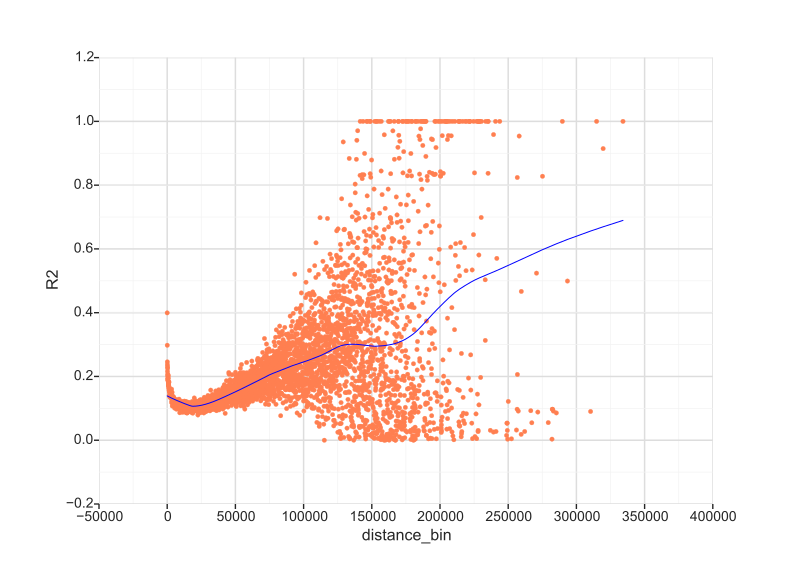
\includegraphics{/home/gus/Documents/YalePostDoc/project_stuff/g_f_fucipes_uganda/ddrad58/manuscript/figures/ld/distance_VS_r2_all.pdf}
\caption{Distance vs \(r^2\) overall}
\end{figure}

\subsubsection{Bin-data membership
quantity}\label{bin-data-membership-quantity}

\textbf{Is the reason for the bizarre data shape due to loss of signal
to noise as shorter contigs are eliminated from data pool?}

\begin{figure}[htbp]
\centering
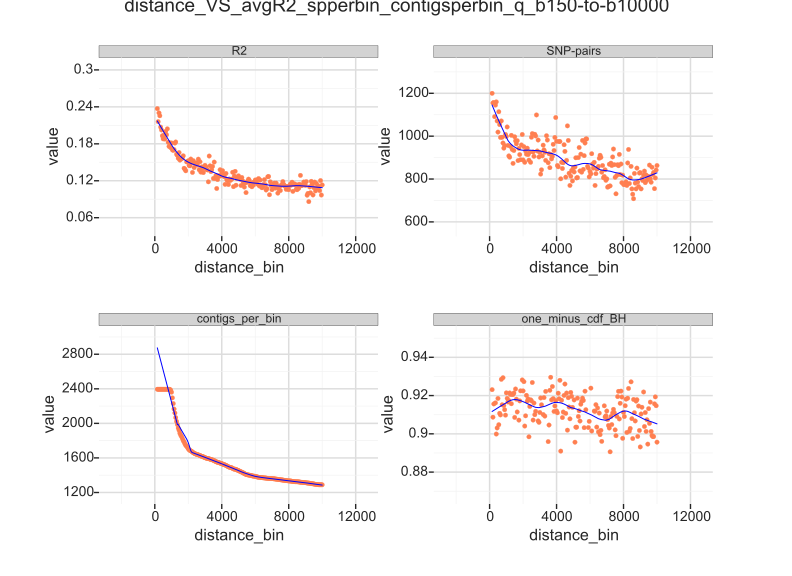
\includegraphics{/home/gus/Documents/YalePostDoc/project_stuff/g_f_fucipes_uganda/ddrad58/manuscript/figures/ld/distance_VS_avgR2_spperbin_contigsperbin_q_b150-to-b10000.pdf}
\caption{Distance vs avg \(r^2\), contigs and \(q\) for bins 150-10000}
\end{figure}

\begin{figure}[htbp]
\centering
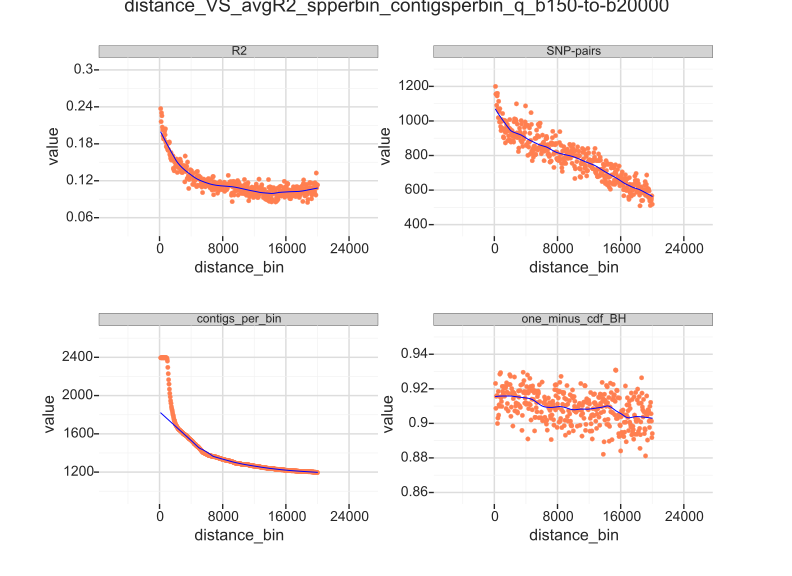
\includegraphics{/home/gus/Documents/YalePostDoc/project_stuff/g_f_fucipes_uganda/ddrad58/manuscript/figures/ld/distance_VS_avgR2_spperbin_contigsperbin_q_b150-to-b20000.pdf}
\caption{Distance vs avg \(r^2\), contigs and \(q\) for bins 150-20000}
\end{figure}

\subsubsection{Bin-data pattern of individual
populations}\label{bin-data-pattern-of-individual-populations}

\section{Dating the North/South population
split}\label{dating-the-northsouth-population-split}

\subsection{Converting the BAMS to NEXSUS for
BEAST}\label{converting-the-bams-to-nexsus-for-beast}

\begin{itemize}
\itemsep1pt\parskip0pt\parsep0pt
\item
  using PGDSpider2 to convert to NEXUS
\item
  BAM location: \texttt{/scratch/ag674/sample\_mappedSC}
\item
  SPID file:
  \href{file:///home/gus/remote_mounts/louise/data/projects/ddrad58/PGDSpider_files/bam_to_nex_for_BEAST/bam_to_nex_for_BEAST.spid}{bam\_to\_nex\_for\_BEAST.spid}
\item
  BAMS to use:

  \begin{itemize}
  \itemsep1pt\parskip0pt\parsep0pt
  \item
    \texttt{find /scratch/ag674/sample\_mappedSC -name \textbackslash{}* \textbar{} grep -P "\textbackslash{}d\textbackslash{}.sorted" \textgreater{} \$HOME/data/projects/ddrad58/PGDSpider\_files/bam\_to\_nex\_for\_BEAST/bam\_to\_nex\_for\_BEAST.bam\_list.txt}
  \item
    \href{file:///home/gus/remote_mounts/louise/data/projects/ddrad58/PGDSpider_files/bam_to_nex_for_BEAST/bam_to_nex_for_BEAST.bam_list.txt}{bam\_to\_nex\_for\_BEAST.bam\_list.txt}
  \end{itemize}
\item
  ref for bam:
  \href{file:///home/gus/remote_mounts/louise/data/genomes/glossina_fuscipes/assemblies/GfusI1/Glossina-fuscipes-IAEA_SCAFFOLDS_GfusI1.fa}{Glossina-fuscipes-IAEA\_SCAFFOLDS\_GfusI1.fa}
\end{itemize}

\subsubsection{2015-03-11 (Wednesday)}\label{wednesday-1}

\begin{itemize}
\itemsep1pt\parskip0pt\parsep0pt
\item
  stymied by permissions issues with the bams.
\item
  see tomorrow
\end{itemize}

\subsubsection{2015-03-12 (Thursday)}\label{thursday}

\paragraph{Attempt 1 {[}FAILED: write
permissions{]}}\label{attempt-1-failed-write-permissions}

\begin{Shaded}
\begin{Highlighting}[]
\KeywordTok{module} \NormalTok{load PGDSpider/2.0.8.0 samtools-bcftools-htslib/1.0}

\KeywordTok{java} \NormalTok{-Xmx2048m -Xms512m -jar /home2/wd238/.local/easybuild/software/PGDSpider/2.0.8.0/PGDSpider2-cli.jar -inputfile /fastscratch/wd238/beast_run/BAMs/KG_10030.sorted.bam -inputformat BAM -outputfile /fastscratch/wd238/beast_run/KG_10030.sorted.bam.nex -outputformat NEXSUS -spid }\OtherTok{$HOME}\NormalTok{/data/projects/ddrad58/PGDSpider_files/bam_to_nex_for_BEAST/bam_to_nex_for_BEAST.spid}
\end{Highlighting}
\end{Shaded}

~\\ \textbf{NOTES:}

\begin{itemize}
\itemsep1pt\parskip0pt\parsep0pt
\item
  \texttt{PGDSpider} seems to write a bunch of temporary files in the
  same dir as the inputfile.
\item
  this breaks because I only have READ access to the data dir
\item
  proceeding with copying the BAMs to a place I have write access to and
  trying again
\end{itemize}

\paragraph{Attempt 2 {[}FAILED: memory
limit{]}}\label{attempt-2-failed-memory-limit}

\begin{Shaded}
\begin{Highlighting}[]
\NormalTok{$ }\KeywordTok{java} \NormalTok{-Xmx2048m -Xms512m -jar /home2/wd238/.local/easybuild/software/PGDSpider/2.0.8.0/PGDSpider2-cli.jar -inputfile /fastscratch/wd238/beast_run/BAMs/KG_10030.sorted.bam -inputformat BAM -outputfile /fastscratch/wd238/beast_run/KG_10030.sorted.bam.nex -outputformat NEXSUS -spid }\OtherTok{$HOME}\NormalTok{/data/projects/ddrad58/PGDSpider_files/bam_to_nex_for_BEAST/bam_to_nex_for_BEAST.spid}

\KeywordTok{-}\NormalTok{[  output   ]-}
\KeywordTok{INFO}  \NormalTok{16:27:47 - load PGDSpider configuration from: /home2/wd238/.local/easybuild/software/PGDSpider/2.0.8.0/spider.conf.xml}
\KeywordTok{initialize} \NormalTok{convert process...}
\KeywordTok{read} \OtherTok{input} \OtherTok{file}\NormalTok{...}
\KeywordTok{INFO}  \NormalTok{16:28:04 - Run samtools/bcftools...}
\KeywordTok{INFO}  \NormalTok{16:28:33 - [bam_sort_core] merging from 3 files...}
\KeywordTok{ERROR} \NormalTok{16:30:24 - not enough memory. To increase the allowed memory see help.}
\KeywordTok{read} \OtherTok{input} \OtherTok{file} \OtherTok{done}\NormalTok{.}
\KeywordTok{write} \NormalTok{output file...}
\KeywordTok{write} \NormalTok{output file done.}
\end{Highlighting}
\end{Shaded}

~\\ \textbf{NOTES:}

\begin{itemize}
\itemsep1pt\parskip0pt\parsep0pt
\item
  \texttt{PGDSpider} ran out of mem.
\item
  I am going to bump up the mem and try again.
\end{itemize}

\paragraph{Attempt 3 {[}FAILED: reference file
issue{]}}\label{attempt-3-failed-reference-file-issue}

\begin{Shaded}
\begin{Highlighting}[]
\NormalTok{$ }\KeywordTok{java} \NormalTok{-Xmx16384m -Xms16000m -jar /home2/wd238/.local/easybuild/software/PGDSpider/2.0.8.0/PGDSpider2-cli.jar -inputfile /fastscratch/wd238/beast_run/BAMs/KG_10030.sorted.bam -inputformat BAM -outputfile /fastscratch/wd238/beast_run/KG_10030.sorted.bam.nex -outputformat NEXSUS -spid }\OtherTok{$HOME}\NormalTok{/data/projects/ddrad58/PGDSpider_files/bam_to_nex_for_BEAST/bam_to_nex_for_BEAST.spid}

\KeywordTok{-}\NormalTok{[  output   ]-}
\KeywordTok{INFO}  \NormalTok{17:23:52 - load PGDSpider configuration from: /home2/wd238/.local/easybuild/software/PGDSpider/2.0.8.0/spider.conf.xml}
\KeywordTok{initialize} \NormalTok{convert process...}
\KeywordTok{read} \OtherTok{input} \OtherTok{file}\NormalTok{...}
\KeywordTok{INFO}  \NormalTok{17:24:16 - Run samtools/bcftools...}
\KeywordTok{INFO}  \NormalTok{17:24:51 - [bam_sort_core] merging from 3 files...}
\KeywordTok{INFO}  \NormalTok{17:26:38 - ...done}
\KeywordTok{ERROR} \NormalTok{17:29:37 - reference file does not contain *!}
\KeywordTok{read} \OtherTok{input} \OtherTok{file} \OtherTok{done}\NormalTok{.}
\KeywordTok{write} \NormalTok{output file...}
\KeywordTok{write} \NormalTok{output file done.}
\end{Highlighting}
\end{Shaded}

~\\ \textbf{NOTES:}

\begin{itemize}
\itemsep1pt\parskip0pt\parsep0pt
\item
  \texttt{PGDSpider} ran out of mem.
\item
  I am going to bump up the mem and try again.
\end{itemize}

\subsubsection{2015-03-13 (Friday)}\label{friday-1}

\begin{itemize}
\itemsep1pt\parskip0pt\parsep0pt
\item
  ABANDONING THIS AND LETTING ARIS TRY TO START FROM SCRATCH via PYRAD.
\item
  thank GAWD.
\end{itemize}

\section{Meeting}\label{meeting}

\begin{itemize}
\itemsep1pt\parskip0pt\parsep0pt
\item
  Introduce Joshua and suggest a meeting
\end{itemize}

\end{document}
